\documentclass[20pt]{article}

\usepackage[english]{babel}
\usepackage[utf8x]{inputenc}
% \usepackage{amsmath}
\usepackage{graphicx}
\usepackage[margin=0.8in]{geometry}

\title{AS205:Ocean Dynamics(Assignment 6)}
\author{Parag Shende}

\begin{document}
\maketitle
\hrule

\section*{Introduction}

We describe the seasonal means of the Ekman transport($M_{x}$ and $M_{y}$) and the Ekman pumping in the Bay of Bengal and Arabian Sea. This is 
undertaken to study the spatial and temporal patterns of the two basins. The seasonal means are constructed for the year 2022.

\section*{Datasets}

The datasets used in this analysis is as follows:

\begin{itemize}
    \item \textbf{Sea Surface Eastward stress} : ASCAT data.
    \item \textbf{Sea Surface Northward stress} : ASCAT data.
\end{itemize}

\section*{Methodology}

The datasets are choosen for the domain of $40^{\circ} E$ to $100^{\circ}E$ and $0^{\circ} N$ to $25^{\circ} N$. This covers the
North Indian ocean. We then calculate the seasonal mean with the following seasons:
\begin{itemize}
    \item \textbf{Summer Monsoon} : June, July, August, September(JJAS)
    \item \textbf{Winter Monsoon} : November, December, January, February(NDJF)
\end{itemize}

The Ekman transport($M_{x}$ and $M_{y}$ both in $\frac{kg}{m s}$) is calculated as follows:
\begin{center}
    $M_{x} = \frac{\tau_{y}}{f}$

    $M_{y} = \frac{-\tau_{x}}{f}$    
\end{center}

where,
$\tau_{x}$ and $\tau_{y}$ are the wind stress(in $\frac{N}{m^{2}}$) in zonal and meridional direction respectively. 

$f$ is the coriolis parameter (in $s^{-1}$). 

The Ekman velocity($w_{E}$ in $m/s$) is calculated as:
\begin{center}
    $w_{E} = - \nabla\times\frac{\vec{\tau}}{\rho f}$
\end{center}

where,
$\rho$ is the density of the water(taken to be $1035 \frac{kg}{m^{3}}$)

\section*{Summer monsoon}

\subsection*{Ekman transport}

\begin{figure}
    \centering
    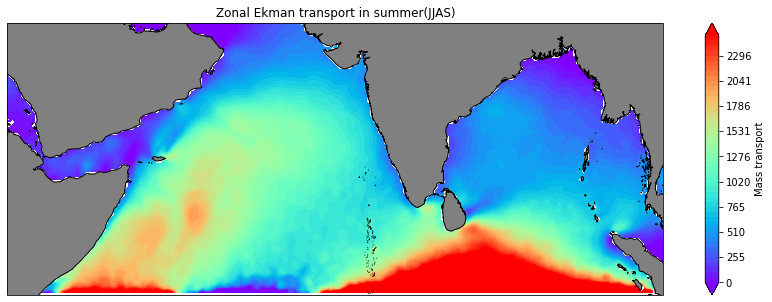
\includegraphics[width=0.88\textwidth]{summer_zonal_trans.png}
    \caption{Zonal Ekman transport in summer in $kg/(m s)$}
\end{figure}

\begin{figure}
    \centering
    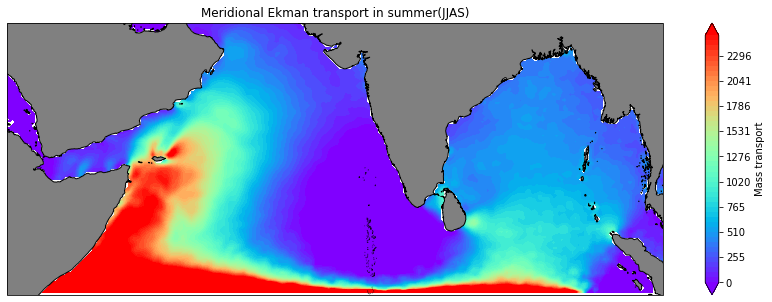
\includegraphics[width=0.88\textwidth]{summer_meridional_trans.png}
    \caption{Meridional Ekman transport in summer in $kg/(m s)$}
\end{figure}

\begin{itemize}
    \item The seasonal mean Ekman transport for summer is plotted in Figure 1 and 2. 
    \item The zonal Ekman transport is maximum along the equator.
    \item The meridional Ekman transport is maximum along the Somali jet region.
\end{itemize}

\subsection*{Ekman pumping}

\begin{figure}
    \centering
    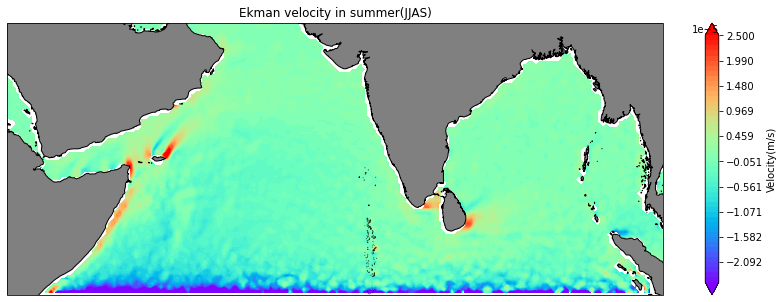
\includegraphics[width=0.88\textwidth]{summer_we.png}
    \caption{Ekman pumping in summer in $m/s$}
\end{figure}

\begin{itemize}
    \item The seasonal mean Ekman velocity for summer is plotted in Figure 3.
    \item There is downwelling along the equator.
    \item Most of the region is dominated by downwelling with isolated spots of upwelling like along Somali coast and eastern coast of Sri Lanka.  
\end{itemize}

\section*{Winter monsoon}

\subsection*{Ekman transport}

\begin{figure}
    \centering
    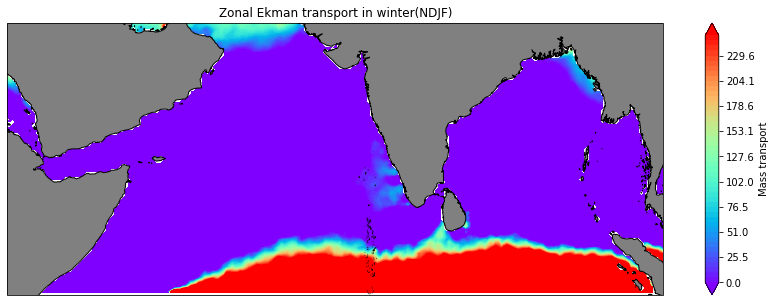
\includegraphics[width=0.88\textwidth]{winter_zonal_trans.png}
    \caption{Zonal Ekman transport in winter in $kg/(m s)$}
\end{figure}

\begin{figure}
    \centering
    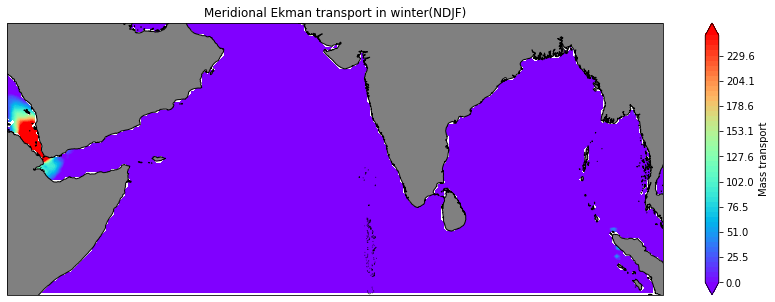
\includegraphics[width=0.88\textwidth]{winter_meridional_trans.png}
    \caption{Meridional Ekman transport in winter in $kg/(m s)$}
\end{figure}

\begin{itemize}
    \item The seasonal mean Ekman transport for winter is plotted in Figure 4 and 5.
    \item There is a significant decrease in meridional Ekman transport in winter, this could be due to weakening of winds. This is majorily southwards.
    \item There is reduction in zonal Ekman transport in winter too owing to similar reason.

\end{itemize}

\subsection*{Ekman pumping}

\begin{figure}
    \centering
    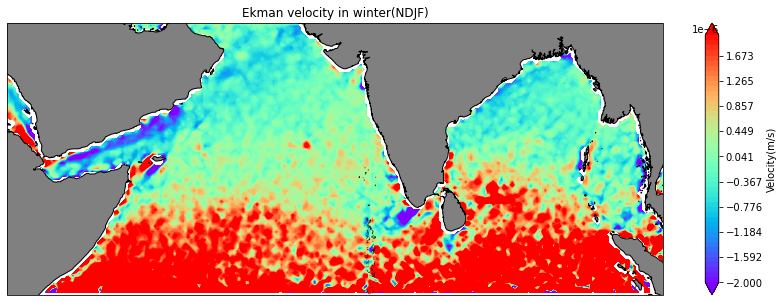
\includegraphics[width=0.88\textwidth]{winter_we.png}
    \caption{Ekman pumping in summer in $m/s$}
\end{figure}

\begin{itemize}
    \item The seasonal mean Ekman velocity for winter is plotted in Figure 6.
    \item There is now upwelling along most of the Southern part of the domain and along equator.
\end{itemize}


\section*{Conclusions}

\begin{itemize}
    \item We compared the seasonal means of zonal and meridional Ekman transport for northern Indian ocean.
    \item Due to weakened winds there is a reduction in Ekman transport in winter.
\end{itemize}

\end{document}